\section{Patterns of Enterprise Application Architecture for Integration (PEAA)}
Patterns of Enterprise Application Architecture for Integration (PEAAI) are a set of design patterns for integrating enterprise applications, written by Martin Fowler. These patterns provide solutions to common integration problems faced in enterprise software development, such as connecting different systems, data migration, and communication between components.

\subsection{Service Layer Pattern}
Define an application's boundary with a layer of services that establishes a set of available operations and coordinates the application's response in each operation.

Other responsibilities of Service Layer:
\begin{itemize}
	\item Role-Based Access Control (RBAC)
	\item Transaction Control, business-level undo (compensation)
	\item Activity logging (e.g. metering, monitoring)
	\item Exception handling
\end{itemize}

\begin{figure}[H]
  \center
  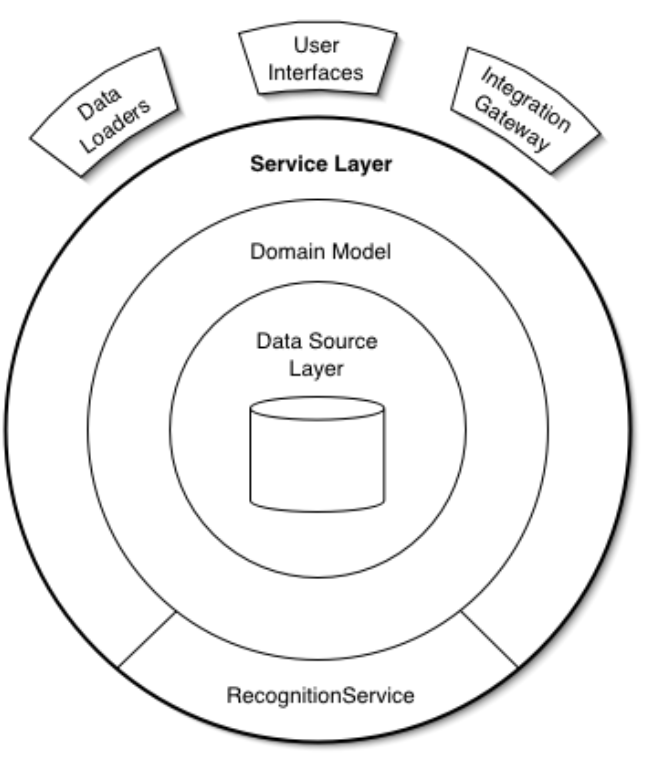
\includegraphics[width=0.45\textwidth]{servicelayerpattern}
  \caption{Service Layer Pattern}
\end{figure}

\subsection{Remote Facade Pattern}
Proves a coarse-grained facade on fine-grained objects to improve efficiency over a network.

\begin{figure}[H]
  \center
  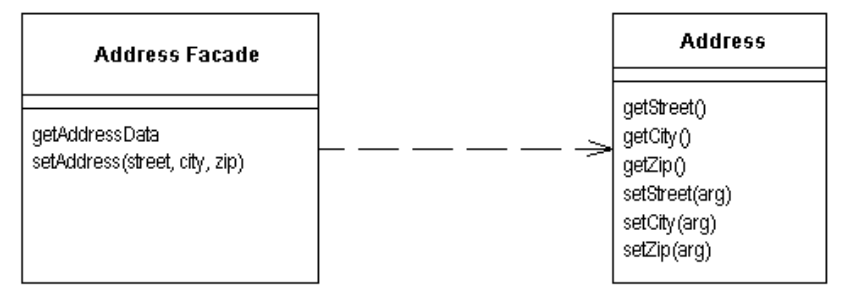
\includegraphics[width=0.5\textwidth]{remotefacade}
  \caption{Remote Facade}
\end{figure}

\subsection{Data Transfer Object (DTO)}
An object that carries data between processes in order to reduce the number of method calls. 

\begin{figure}[H]
  \center
  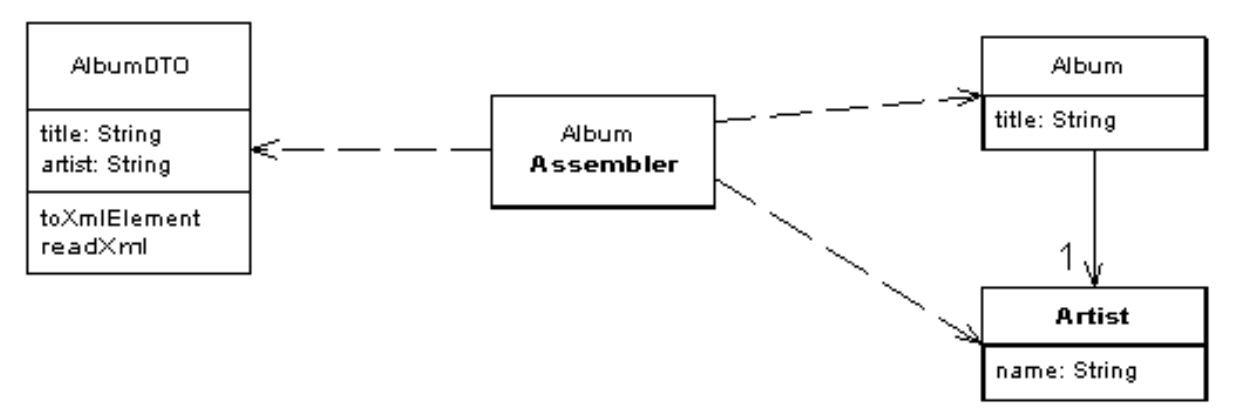
\includegraphics[width=0.75\textwidth]{datatransferobject}
  \caption{Data Transfer Object}
\end{figure}

\section{Service-Oriented Architecture (SOA)}
Mostly consists of separating your application into multiple services (most commonly HTTP services) which can be classified as different types like subsystem or tiers. There is not a single definition for SOA, since it means different things to people. A microservices architecture is a further evolution of SOA.

\begin{itemize}
	\item A set of services and operations that a business wants to expose to their customers and partners, or other portions of the organization.
	\item An architectural style which requires a service provider, a service requestor (consumer) and a service contract (a.k.a. client/server).
	\item  A set of architectural patterns such as service layer (with remote facades, data transfer objects), enterprise service bus, service composition (choreography/orchestration), and service registry, promoting principles such as modularity, layering, and loose coupling to achieve design goals such as reuse, and flexibility.
	\item  A programming and deployment model realized by standards, tools and technologies such as Web services (WSDL/SOAP), RESTful HTTP, or asynchronous message queuing (AMQP etc.)
\end{itemize}

\begin{figure}[H]
  \center
  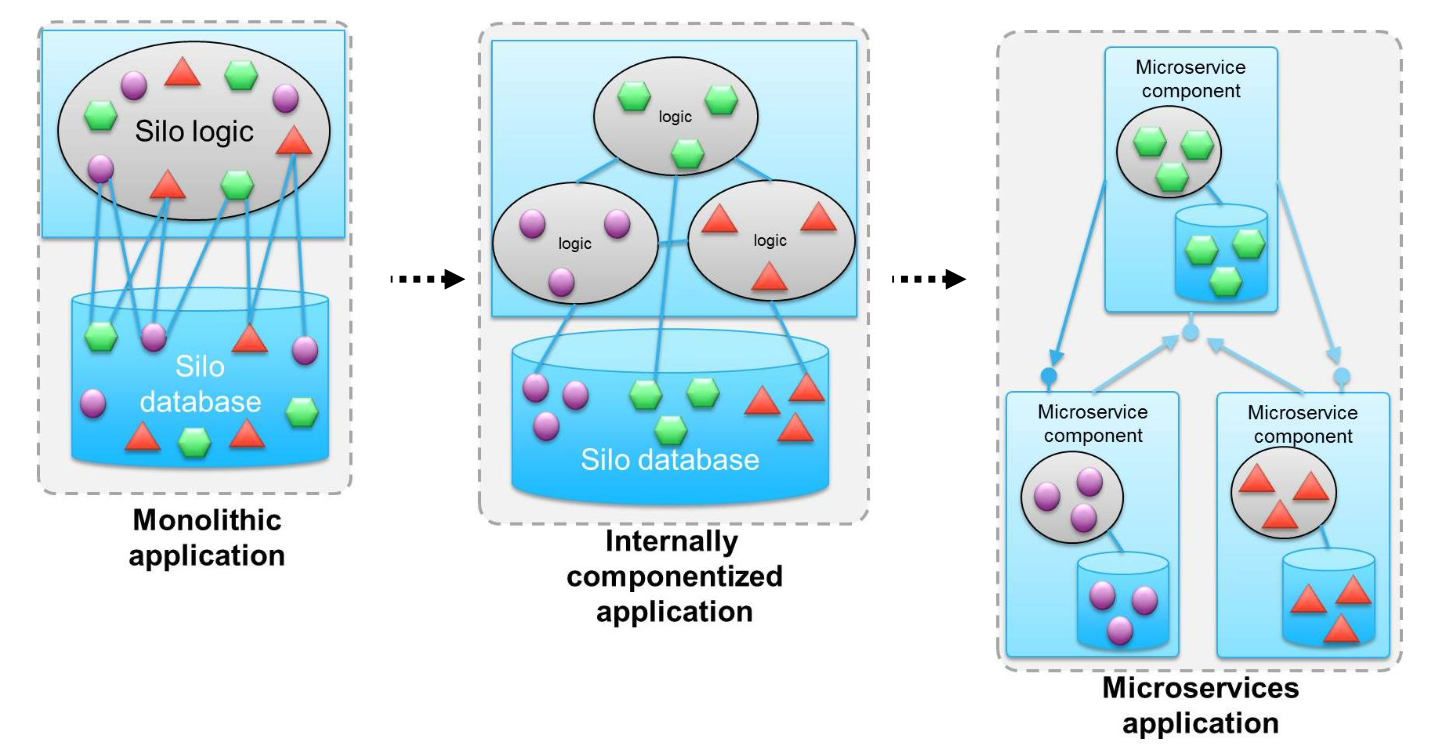
\includegraphics[width=0.75\textwidth]{soa}
  \caption{From Monolith and Components to SOA and MicroServices}
\end{figure}

\subsection{Microservices}
Microservices architectures evolved from previous incarnations of Service-Oriented Architectures (SOAs) to promote agility and elasticity. Microservices are independently deployable, scalable and changeable services each having a single responsibility. These are often deployed in lightweight containers, encapsulate their own state, and communicate via message-based remote APIs (HTTP, queueing), ideally in a loosely coupled fashion.

\subsubsection{Benefits of Microservices}
\begin{itemize}
  \item They support agile development practices with continuous delivery and deployment. Ex. each microservice is owned by a single team, which allows each team to independently develop, deploy and operate their respective service.
  \item They are well suited for implementing ‘IDEAL’ cloud-native applications (i.e., \textbf{isolated} state, \textbf{distributed}, \textbf{elasticity}, \textbf{automated} management, \textbf{loose} coupling). When deployed independently, horizontal on-demand scalability can be achieved through container virtualization and elastic load balancing.
  \item They allow an incremental migration of monolithic applications, which reduces the risk of failure of software modernization efforts.
\end{itemize}

\subsubsection{Challenges of Microservices}
\begin{itemize}
  \item The communication overhead within a distributed architecture combined with poor API design choices can impact the performance of microservice architectures.
  \item Scaling the architecture to include a large number of microservices requires a disciplined approach to their life cycle management, monitoring, and debugging.
  \item Single points of failure and cascading failure proliferation effects need to be avoided, for example through redundancy or circuit breakers. This reduces the risk that failing downstream microservice instances bring down upstream ones (and, eventually, the entire system).
  \item Data consistency and state management challenges are introduced, for example when decoupling monolithic, stateful applications into independent, autonomous microservices (Furda et al. (2018)).
Autonomy and consistency for the whole microservice architecture cannot be both guaranteed when employing a traditional backup and disaster recovery strategy
\end{itemize}

\section{Representational State Transfer (REST)ful HTTP}
REST is an architectural style (for integration), defined via constraints. There it is not an API technology or protocol. RESTful HTTP is one prominent incarnation of this style, when it is done right. 

\begin{itemize}
	\item Client-Server
	\item Stateless
	\item Cacheable
	\item Uniform Interface (URI, HTTP)
	\item Layered System
	\item Code on Demand (Optional)
\end{itemize}

\begin{figure}[H]
  \center
  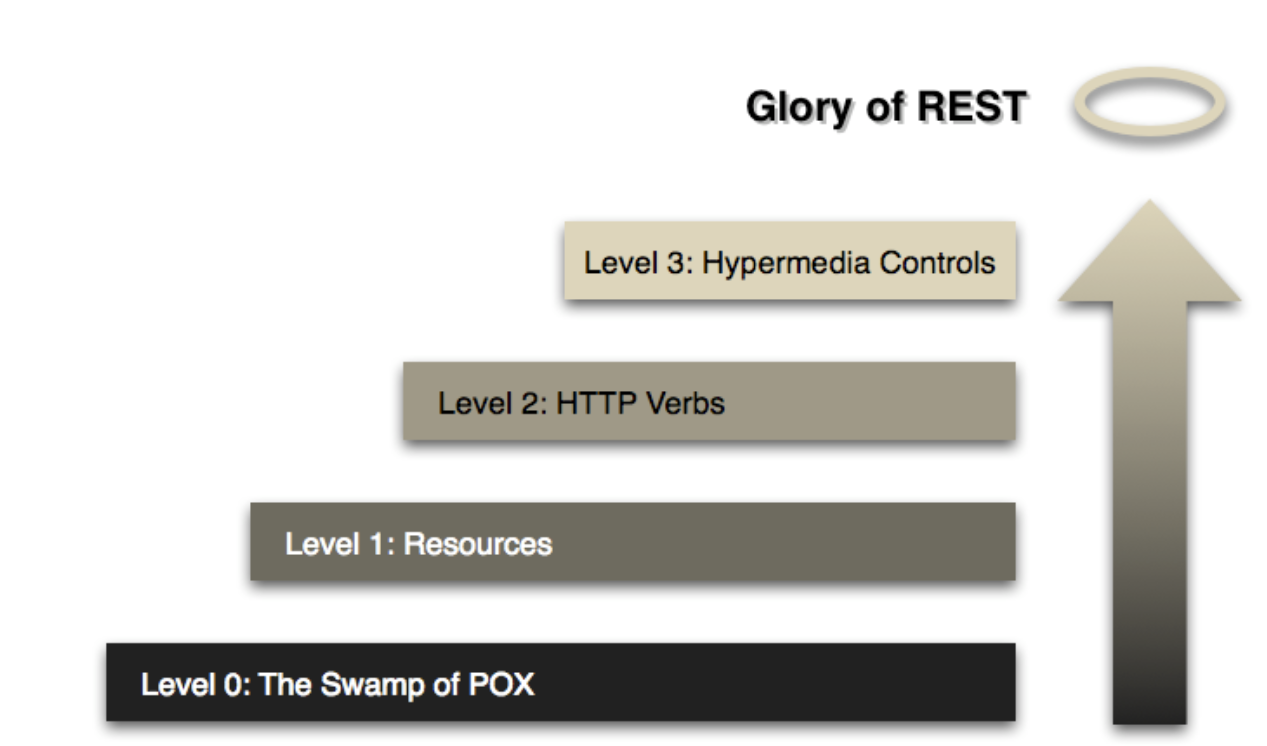
\includegraphics[width=0.5\textwidth]{rest}
  \caption{The Glory of REST}
\end{figure}

\subsection{Hypermedia as the Engine of Application State (HATEOAS)}
Before we can grasp the definition of HATEOAS we need to have some parts defined. HATEOAS is a part of RESTful API architecture and design. HATEOAS make the APIs self-descriptive. Therefore the consumer does not need to know everything about the API.

\begin{description}
	\item [Hypermedia] are links to different parts of the API. These links are documentation and teaches the developer on how to use the API. 
\end{description}

The following listing shows a JSON http answer with the hypermedia links which provide further actions. 

\begin{lstlisting}
HTTP/1.1 200 OK
Content-Type: application/+json
Content-Length: ...
{
   "payroll": {
       "employee_number": "employee_123",
       "salary" : 1000,
       "links": {
           "increment": "/payroll/employee_123/increment",
           "decrement": "/payroll/employee_123/decrement",
           "close": "/payroll/employee_123/close"
       }
   }
}
\end{lstlisting}

\subsection{HTTP and REST}
HTTP protocol primitives: sent by client, understood by server, client e.g. web browser.

\begin{figure}[H]
  \center
  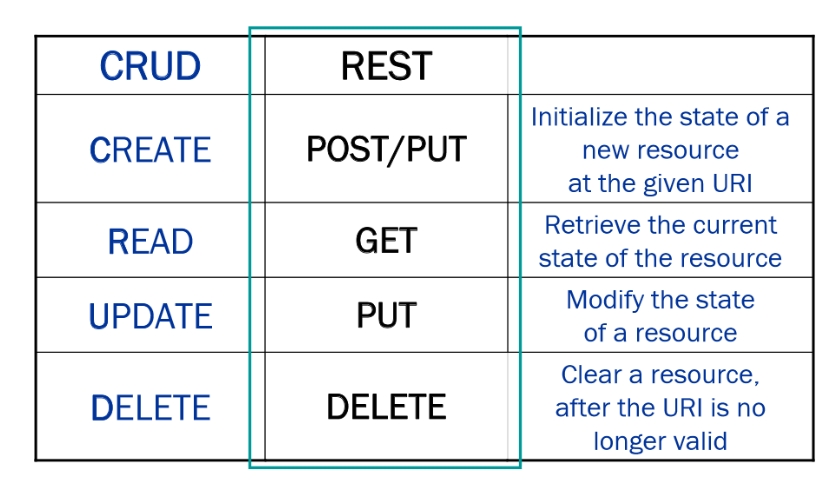
\includegraphics[width=0.5\textwidth]{httpandrest}
  \caption{REST Verbs}
\end{figure}


